\section{A Uniqueness Theorem for Clustering}

\subsection*{Introduction}

Recall from class Kleinberg's impossibility result, which states that a clustering algorithm cannot satisfy the three axioms of \textbf{scale-invariance}, \textbf{richness}, and \textbf{consistency} simultaneously. This gives some insight on why most clustering algorithms seem to be inadequate for some applications. Recall the definitions of the axioms:

Let $X$ be a set of points and $d$ be some distance metric. Then let $f(X,d) \rightarrow P$ be a clustering algorithm which partitions $X$ into some clusters $P$

\begin{definition}
    $f$ satisfies \textbf{Scale Invariance} if:
    $$
    f(X, d) = f(X, \alpha d) \ \  \forall \alpha > 0
    $$
\end{definition}

\begin{definition}
    $f$ satisfies \textbf{Richness} if for all possible partitions $P$ of $X$, there exists some $d$ such that:
    $$
    f(X, d) = P
    $$
\end{definition}

\begin{definition}
    $f$ satisfies \textbf{Consistency} if given a partitioning $P$ arising from a distance metric $d$, then for any other metric $d'$ that enhances the partition ($d' \leq d$ for intra-cluster distances, and $d' \geq d$ for inter-cluster distances) we have:
    $$
    f(X,d) = f(X,d') = P
    $$
\end{definition}

While it is impossible to satisfy all three of these axioms simultaneously, by relaxing these axioms a bit, we can come up with a clustering algorithm that satisfies the relaxed axioms. Moreover, in a paper by Reza Bosagh Zadeh and Shai Ben-David, they propose some additional abstract properties of clustering algorithms and obtain a uniqueness theorem, showing that only the Single-Linkage algorithm satisfies the resulting set of properties.


\newpage


\subsection*{Single-Linkage \& Uniqueness Theorem}

Firstly, we outline the Single-Linkage clustering algorithm:

\begin{center}
    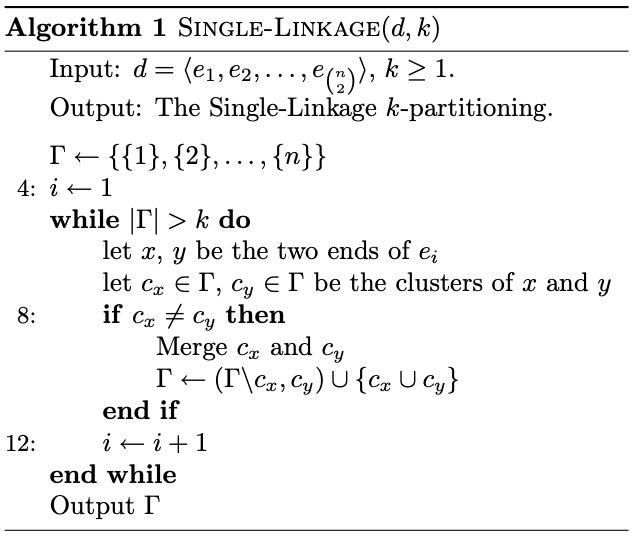
\includegraphics[width = 10cm]{chapter_4/files/single_linkage.png}
\end{center}

The input for the algorithm is an \textit{ordered} list of edge weights (pairwise distances between points provided by $d$), and the number of clusters $k$. The overall idea of the algorithm is to construct a MST of the data, and then remove the $k-1$ most expensive edges to leave $k$ connected components which are the clusters.

\medskip

Next, we outline the relaxed modifications of Kleinberg's axioms, which is just adding the criterion that the number of clusters $k$ is given a part of the input. Thus, in all the axioms, the number of possible partitions is restricted to partitions of $k$ clusters. We redefine the clustering algorithm as $F$, which implicitly acts on an input of points, thus removing $X$ as a parameter.

\begin{definition}
    F satisfies \textbf{k-Richness} if for all possible partitions $P$ of $X$ of size $k$, there exists some $d$ such that:
    $$
    F(d, k) = P
    $$
\end{definition}

The definition of \textbf{Consistency} is also modified to limit all partitions $P$ to be of size $k$, a constant which is fixed beforehand.

\medskip

In additional, Zadeh and Ben-David propose two more properties: \textbf{Order-Consistency} and \textbf{MST-Coherence}. Firstly, we will define order-consistency:

\begin{definition}
    $F$ satisfies \textbf{Order-Consistency} if for any two distance functions $d$ and $d'$, number of clusters k, if the order of edges in $d$ is the same as the order of edges in $d'$, then 
    $$
    F(d, k) = F(d', k)
    $$
\end{definition}


\begin{theorem}
    Single-Linkage (SL) satisfies \textbf{Scale Invariance}, \textbf{k-Richness}, \textbf{Consistency}, and \textbf{Order-Consistency}
\end{theorem}

\begin{proof}
    
    SL satisfies Order-Consistency because the algorithm only compares the lengths of the edges, so as long as the order of the edges remains the same, the algorithm will run the same. Satisfying Order-Consistency implies Scale Invariance.
    
    SL satisfies $k$-Richness because for any partition $P$, we can define $d$ such that all inter-cluster distances are $2$ and all intra-cluster distances are $1$; SL will then return $P$.
    
    The proof that SL satisfies Consistency can be seen by considering the edge weights $d$, and doing a case analysis on what happens if each intra-cluster edge is shrunk, and each inter-cluster edge is expanded.
    
\end{proof}

Consistency, Scale Invariance, and $k$-Richness do not uniquely determine the
Single-Linkage algorithm since Min-Sum $k$-centers also satisfies all three axioms. To uniquely define Single-Linkage, we introduce the property of MST-Coherence. Let $MST(d)$ be the minimum spanning tree of the graph induced by the distance metric $d$, as output by Kruskal's algorithm.

\begin{definition} $F$ satisfies \textbf{MST-Coherence} if d and $d'$ are distance functions such that $MST(d) = MST(d')$, then for all k, 
    $$
    F(d, k) = F(d, k')
    $$
\end{definition}

MST-Coherence basically forces clustering algorithms to ignore redundant edges in clustering; which is performed on line 8 of the SL algorithm. It is important to note that we do \textit{not} expect all clustering algorithms to satisfy MST-Coherence, and thus it is not referred to as an axiom. 

\begin{theorem}
    Single-Linkage satisfies \textbf{k-Richness}, \textbf{Consistency}, \textbf{Order-Consistency}, and \textbf{MST-Coherence}
\end{theorem}

\begin{proof}
    Follows directly from the definition of MST-Coherence, and the definition of the SL algorithm provided. Note Scale Invariance is omitted due to being implied by Order-Consistency.
\end{proof}

Now, we begin the proof of the Uniqueness Theorem. Firstly, we want to ensure our properties do not implicitly characterize Single-Linkage. We define a property to be \textit{necessary} if three of the four above properties are not sufficient to describe Single-Linkage

\begin{theorem}
    Consistency, and k-Richness are necessary to characterize Single-Linkage
\end{theorem}

\begin{proof}
    For each property, we will show another clustering algorithm different to SL that also satisfies the three other properties.
    
    Define the \textbf{Minimum Spanning Tree Cuts} (MSTC) procedure: Given $n$ points and constant $k$, produce a MST of the $n$ points. Then, cut $k-1$ edges of the MST defined by $C_k$, where $|C_k| = k-1$, and each entry $c \in C_k; c \in \mathbb{N}; 1 \leq c \leq n-1$ directs the $c^{th}$ most expensive edge to be cut. For example, in SL, we cut the most expensive edges so $C_k = \{n-1, n-2, \cdots, n-k+1\}$.
    
    All MSTC clustering algorithms are MST-Coherent, Order-Consistent, and $k$-Rich; the first two can be verified from the definition of the MSTC procedure (it uses a MST, and only uses the order of the edges), and $k$-richness is proven using the a similar method as we for SL (setting all edge weights to 1 or 2 corresponding to the elements of $C_k$ to give a desired partition).
    
    \textit{Consistency is necessary}. If we take $C_k = \{1, 2, \cdots , k-1\}$, we are able to verify that the resulting MSTC clustering algorithm will be inconsistent.
    
    \textit{k-Richness is necessary}. Consider the Constant clustering algorithm which always returns the first $n-k+1$ elements of S as a single cluster and returns the remaining $k-1$ elements as singleton clusters with one point inside each cluster, making a total of $k$ clusters. This algorithm does not look at $d$, so is clearly MST-Coherent, Order-Consistent, and Consistent. However, it is clearly not $k$-Rich because we can never return a clustering which has no singleton clusters.
    
\end{proof}

Next, we prove a Lemma which will be important in our proof of Uniqueness. Define an edge $e$ as an \textit{inner edge} if both ends of $e$ are in the same cluster. Conversely, $e$ is an \textit{outer edge} if the ends of $e$ are in different clusters. The lemma shows that under some conditions, we can maintain clustering even if we switch the order of edges.

\begin{lemma}
    Given a Consistent partitioning algorithm $F$, and a distance function $d$ with edges in ascending order of weight 
    $$
    d = \langle e_1, e_2, \cdots, e_p, e_q, \cdots e_{\binom{n}{2}} \rangle
    $$
    then for all $k > 0$, if $e_p$ and $e_q$ are both inner edges or both outer edges (w.r.t. $F(d, k)$), we have
    $$
    F(\langle e_1, e_2, \cdots, e_q, e_p, \cdots e_{\binom{n}{2}} \rangle
    $$
\end{lemma}

\begin{proof}
    The proof comes directly from the definition of consistency; if $e_p$ and $e_q$ are both inner edges, we can keep shrinking $e_q$ until $e_q < e_p$; conversely, if they are both outer edges, we can expand $e_p$ until $e_q < e_p$.
\end{proof}

This leads us to our Uniqueness Theorem:

\begin{theorem}
    Single-Linkage is the only Consistent, k-Rich, MST-Coherent, Order-Consistent partitioning algorithm.
\end{theorem}

\begin{proof}
    Let $F$ be any Consistent, $k$-Rich, MST-Coherent partitioning algorithm, and let $d$ be any distance function on $n$ points. We want to show that that for all $k > 0$, $F(d, k) = SL(d, k)$. Let $SL(d,k) = \Gamma$, and let inner and outer edges be defined w.r.t $\Gamma$. Let the ordering of the edges under $d$ be $e^* = \langle e_1, e_2, \cdots, e_{\binom{n}{2}} \rangle$, and define $e^*_i$ to be the same ordering under distance $d_i$.
    
    By $k$-Richness, there exists some $d_1$ such that $F(d_1,k) = \Gamma$. We will aim to transform $d_1$ to get $d$, while preserving the clustering $\Gamma$. 
    
    Because Single-Linkage removes only the most expensive edges, there is a prefix of edges $p = \langle e_1, e_2, \cdots, e_t \rangle$ that are all inner edges, that by themselves define the clustering of $\Gamma$ (all other inner edges are implicitly given because they are connected via $p$.
    
    Define a \textit{redundant inner edge} to mean all inner edges not in $p$; equivalently, all redundant inner edges have weight greater than some outer edge. Note that we can increase the weights of any redundant inner edge without affecting the MST, and thus increasing the weights of redundant inner edges does not affect the clustering $\Gamma$ since $F$ is MST-Coherent.
    
    We outline the transformation of $d_1$ to $d$:
    \begin{enumerate}
        \item $d_1$ is defined such that $F(d_1,k) = \Gamma$
        \item Shrink all edges in $p$ until they become the $t$ shortest edges. This does not affect $\Gamma$ since $F$ is Consistent, and we are only shrinking intra-cluster distances. Call this distance $d_2$
        \item Reorder the first $t$ edges of such that the edges are in the same order as $e^*$. Since all the edges are inner edges, rearranging them makes no difference to $\Gamma$ by Lemma 4. Call this distance $d_3$. Thus, the first $t$ edges in $e^*_3$ are the same (in identity) to the first $t$ edges in $e^*$
        \item Expand all outer edges until they are larger than all inner edges (even redundant ones). $\Gamma$ does not change by Consistency. Call this distance $d_4$
        \item Reorder all the outer edges until they are in the same order as in $e^*$; again this does not affect $\Gamma$ by Lemma 4. Call this distance $d_5$
        \item Now we need to put the redundant inner edges in their correct order in $e^*$. By MST-Coherence, if we just expand these edges by any amount, the MST will not change and thus $\Gamma$ remains the same. Let the distance after doing this be $d_6$.
        \item The edges are now in the same order as they would be under $d$, but they may not have the same weights. By Order-Consistency, we can adjust the weights as much as we want as long as we do not change the order, and maintain $\Gamma$. We adjust the edge weights to make them identical to $d$. Let this final distance be $d_7$
    \end{enumerate}
    
    We have $F(d_7,k) = F(d,k) = \Gamma = SL(d, k)$, so Single-Linkage must be the unique Consistent, k-Rich, MST-Coherent, Order-Consistent partitioning algorithm.
\end{proof}